\begin{document}

\maketitle

\section{1184095 Dian Markuci}
\subsection{Teori}
	\subsubsection{Sejarah Perkembangan dan Definisi Artificial Intelligence}      
	
	\begin{enumerate}
	    \item  Kecerdasan Buatan atau \textit{Artificial Intelligence} (AI) merupakan teknik meniru kecerdasan yang dimiliki baik makhluk hidup maupun benda mati untuk menyelesaikan sebuah masalah. Atau bisa di definisikan sebagai salah satu cabang Ilmu pengetahuan yang berkaitan dengan pemanfaatan mesin untuk menyelesaikan persoalan rumit menggunakan cara yang lebih manusiawi.
	    
	    \item  Pada tahun 1956 inilah pertama kali muncul istilah AI atau Artificial Intellegent. Penggunaan AI begitu popular dari tahun ke tahun. Pada tahun 1950 -an merupakan tahap riset awal proyek AI yang tujuan untuk eksplorasi topik penyelesaian persoalan dan metode simbolik. Selanjutnya pada tahun 1960 an Departemen Pertahanan yang berasal dari Amerika Serikat memiliki keinginan dalam melatih dan mengembangkan komputer agar memiliki nalar yang menyerupai manusia secara dasar. Pada tahun 1970 -an, adanya keberhasilan proyek DARPA (Defence Advanced Research Project Agency) dengan mampu menyelesaikan studi kasus tentang pemetaan jalan. Selanjutnya awal abad ke – 21, atau lebih tepat di tahun 2003, DARPA berhasil untuk menciptakan asisten pribadi cerdas. Sejak saat itu, teknologi AI terus berkembang sampai saat ini dan lebih menjurus pada program yang lebih detail dan kompleks, dengan penerapan algoritma dari pembelajaran secara mendalam atau deep learning yaitu AI yang dikembangkan bisa mengerjakan persoalan dan memberi solusi yang lebih kompleks dengan kondisi yang lebih beragam.
	\end{enumerate}
    
    

    \subsubsection{Supervised learning, Klasifikasi, Regresi dan unsupervised learning. Data set, Training set dan Testing set}
    
    \begin{enumerate}
    
    \item Supervised learning adalah suatu pembelajaran dengan adanya pengawas atau bisa di sebut ada supervisornya. Supervisor disini berarti suatu label yang ada di setiap data nya. Kemudian maksud label tersebut adalah tag dari data yang ditambah ke dalam model pembelajaran mesin atau lebih trend di sapa machine learning model. Bisa diilustrasikan misal seperti gambar pepaya di tag “pepaya” di masing masing gambar pepaya dan gambar paprika di tag “paprika” di masing masing gambar paprika. Machine learning kategori dapat berupa clasification (“pepaya”, “paprika”, dsb) dan regression ( tinggi badan, berat badan, dsb). 

    \item Klasifikasi dan Regresi
Cara kerja supervised learning dalam ilustrasi ini dibagi menjadi dua yaitu klasifikasi dan regresi. Mesin dapat mengelompokan data sesuai klasifikasinya. Kemudian regresi mampu mengidentifikasi data nyata berupa angka seperti tinggi, berat, ataupun dollar. Dalam dunia data science supervised learning merupakan algoritma yang lebih sering digunakan dibandingkan dengan unsupervised learning. Di supervised learning, terlebih dahulu algoritma akan seolah-olah dilatih agar bisa melakukan prediksi ataupun klasifikasi. Kemudian Data Scientist lah yang seolah-olah bertindak menjadi seorang supervisornya yang melatih algoritma tersebut. 

\item Unsupervised Learning
\par
Unsupervised learning adalah suatu pembelajaran tanpa adanya pengawas dan tidak menggunakan label untuk bisa memprediksi target variable. Unsupervised learning mengelompokan dengan kesamaan ataupun kemiripan dari attribut attribut yang diinputkan. Apabila attribut dan sifat dari data variable yang diproses ternyata memiliki kemiripan, maka akan di jadikan satu kelompok (clustering). Maka akan menimbulkan beberapa bagian kelompok (cluster). Jumlah cluster bisa tidak terbatas. Dari kelompok kelompok tersebut model melabelkan, dan jika data baru akan di prediksi, itu akan diproses untuk mencocokan kelompok yang memiliki kemiripan feature. unsupervised learning tidak punya outcome spesifik seperti supervise learning karena tidak adanya label dasar.

\item{Data Set}
Dalam membangun sebuah model dengan Pembelajaran mesin, dataset  adalah salah satu hal utama yang penting dan dibutuhkan. Sebelum memulai dengan algoritma apapun, seseorang harus punya pemahaman yang baik mengenai data. Pada dasarnya dataset digunakan untuk mencapai tujuan sebuah penelitian. kemudian sebagian besar kumpulan data ini sifatnya homogen. Data digunakan untuk melatih dan untuk mengevaluasi model yang akan dihasilkan.

\item{Training Set}
Data yang digunakan untuk bisa melakukan klasifikasi ataupun prediksi. Dengan data training maka akan didapatkan sebuah model regresi yang selanjutnya akan digunakan untuk melakukan prediksi.

\item{Testing Set}
Data yang digunakan untuk menguji kebenaran model. Testing data berisi unseen example dimana merupakan contoh yang tidak ada di training set.
	\end{enumerate}
	
\subsection{Praktek}
\subsubsection{Instalasi}
\begin{enumerate}
		\item Langkah pertama yaitu instalasi library scikit pada anaconda, ketik " pip install -U scikit-learn " pada terminal anaconda. 

		\begin{figure}[H]
		\centering
		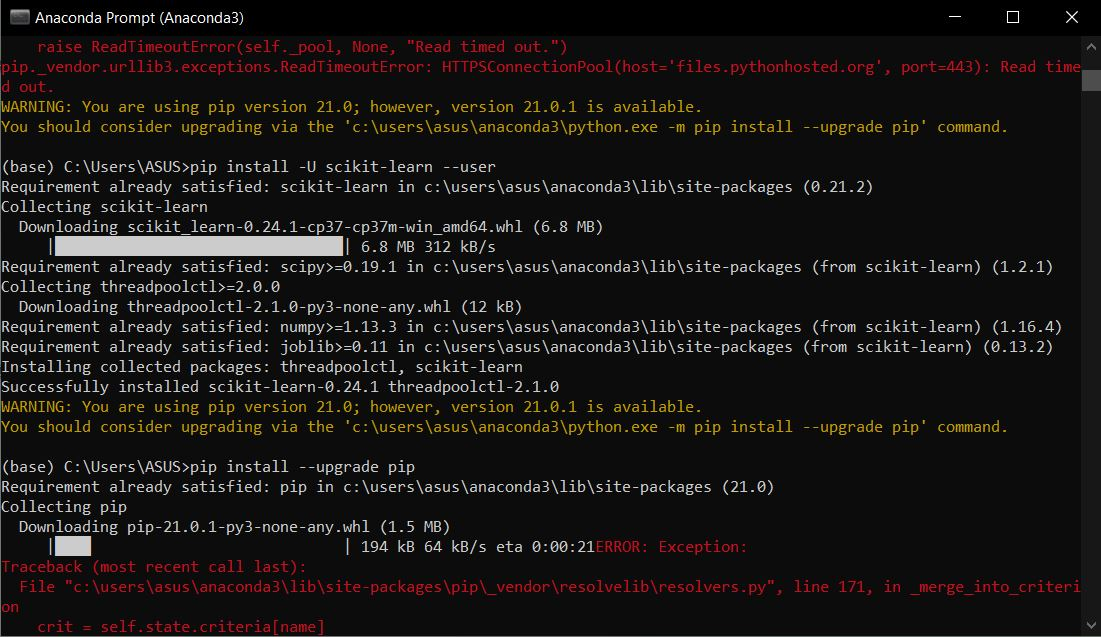
\includegraphics[width=1\textwidth]{figures/1184095/chapter1/Capture.JPG}
		\caption{Instalasi Scikit Learn}
		\label{print}
		\end{figure}
		
        \item{Beres instalasi, pilih satu example dari website Scikit}
        \begin{figure}[H]
		\centering
		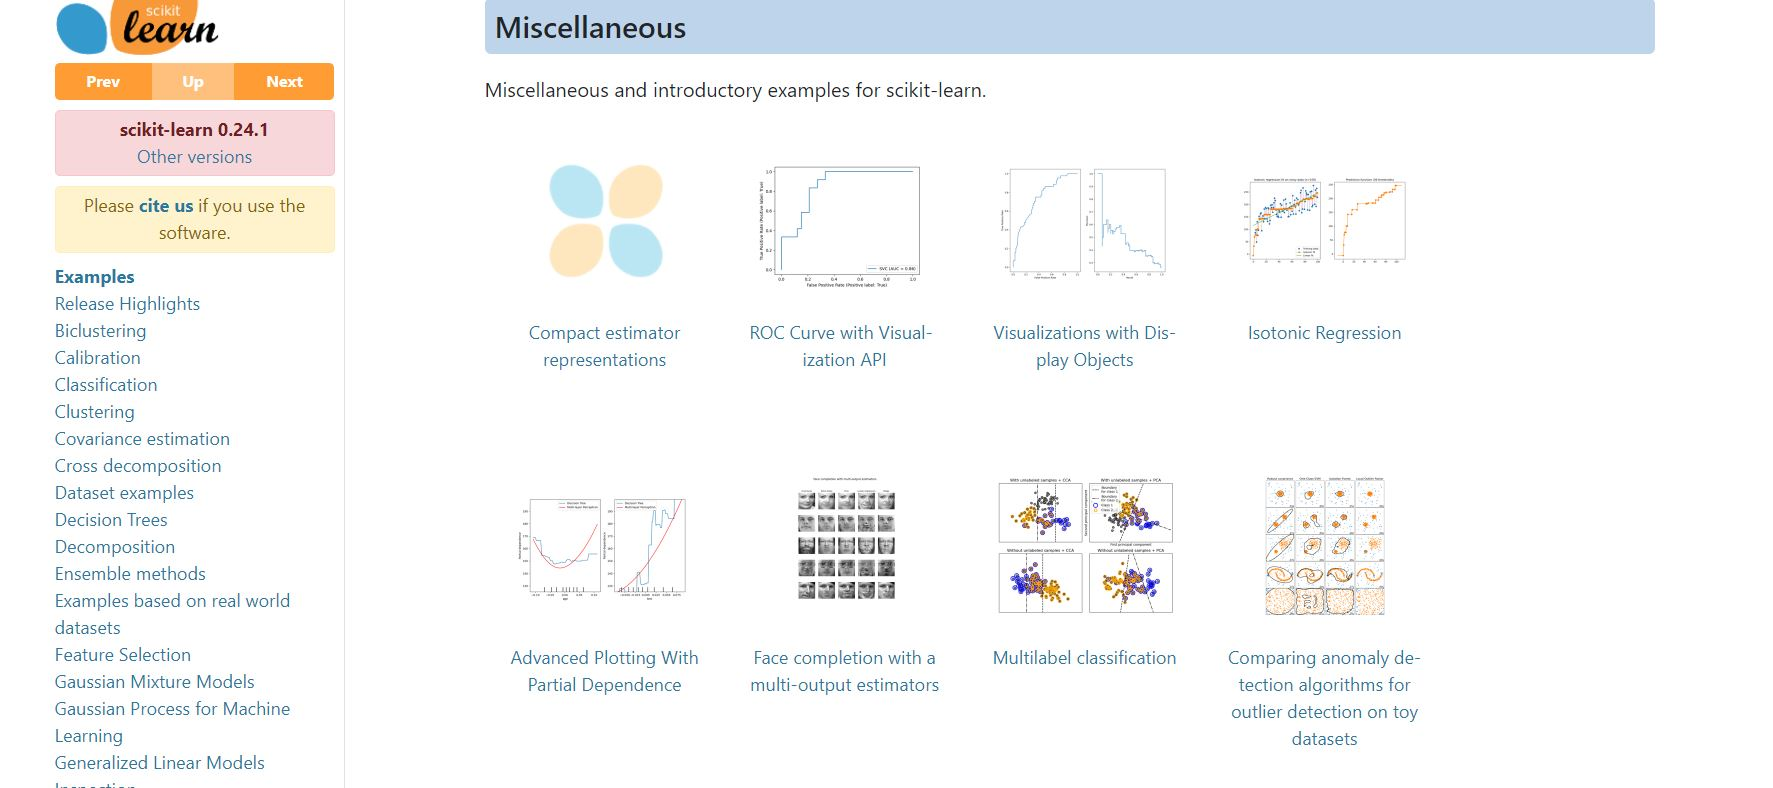
\includegraphics[width=1\textwidth]{figures/1184095/chapter1/4.JPG}
		\caption{website scikit}
		\label{print}
		\end{figure}
		
		\item{Jalankan example yang sudah dipilih di spyder dan lihat hasilnya}
        \begin{figure}[H]
		\centering
		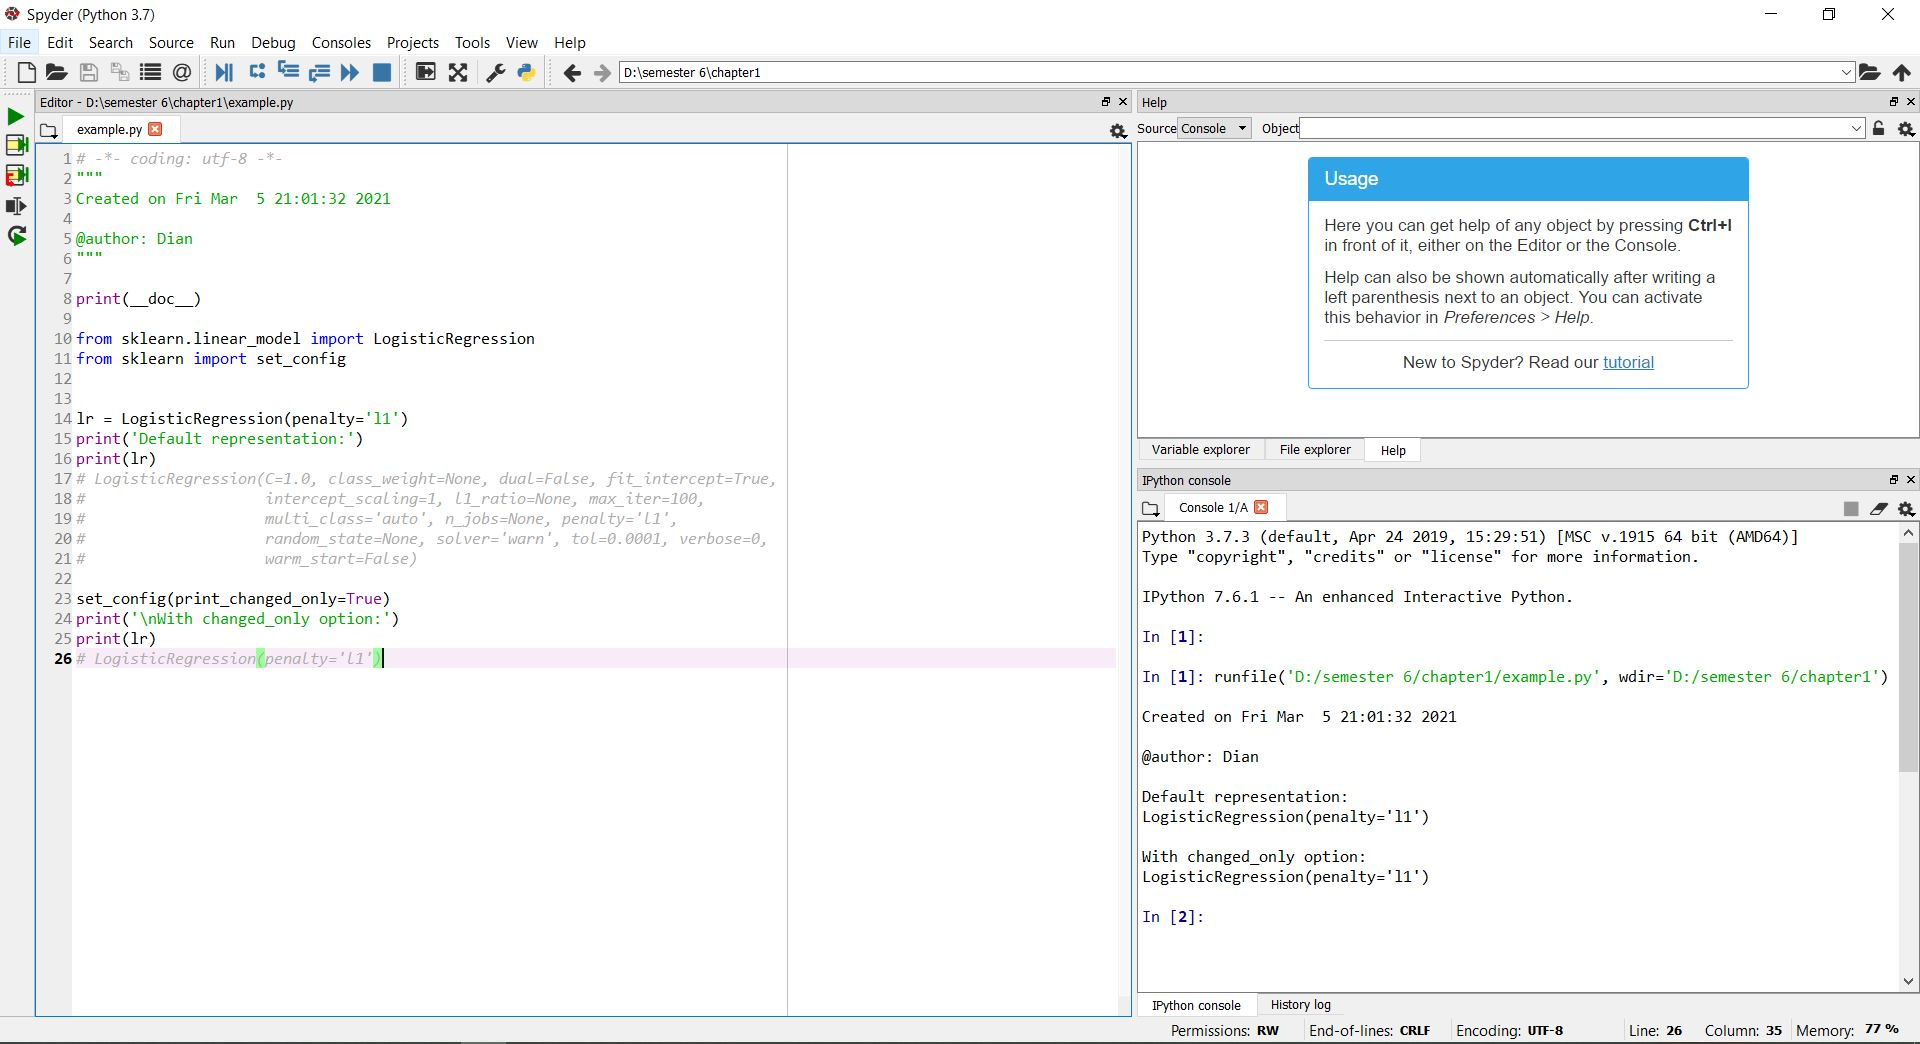
\includegraphics[width=1\textwidth]{figures/1184095/chapter1/5.JPG}
		\caption{example}
		\label{print}
		\end{figure}
		
		\item{Beres instalasi, pilih satu example dari website Scikit}
        \begin{figure}[H]
		\centering
		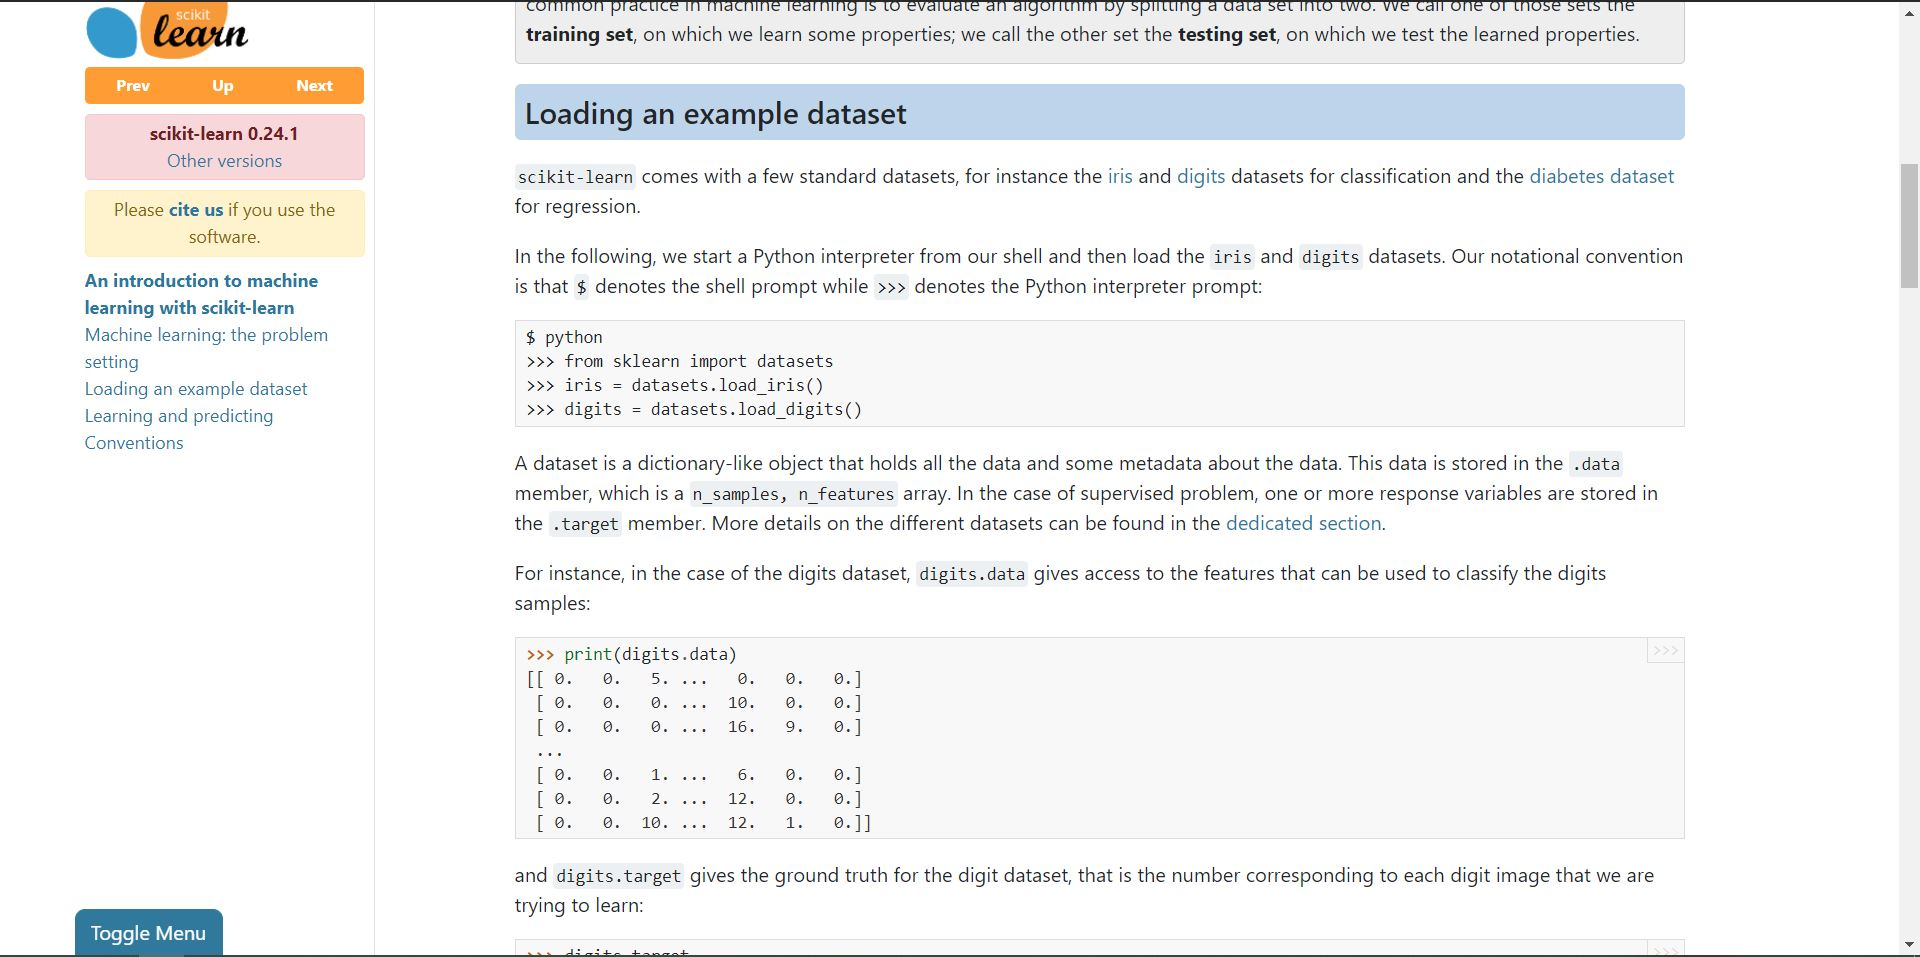
\includegraphics[width=1\textwidth]{figures/1184095/chapter1/6 awal.JPG}
		\caption{website scikit}
		\label{print}
		\end{figure}
		
		\item{latihan selanjutnya mencoba Loading an example dataset, Jalankan kodenya dan lihat hasilnya}
        \begin{figure}[H]
		\centering
		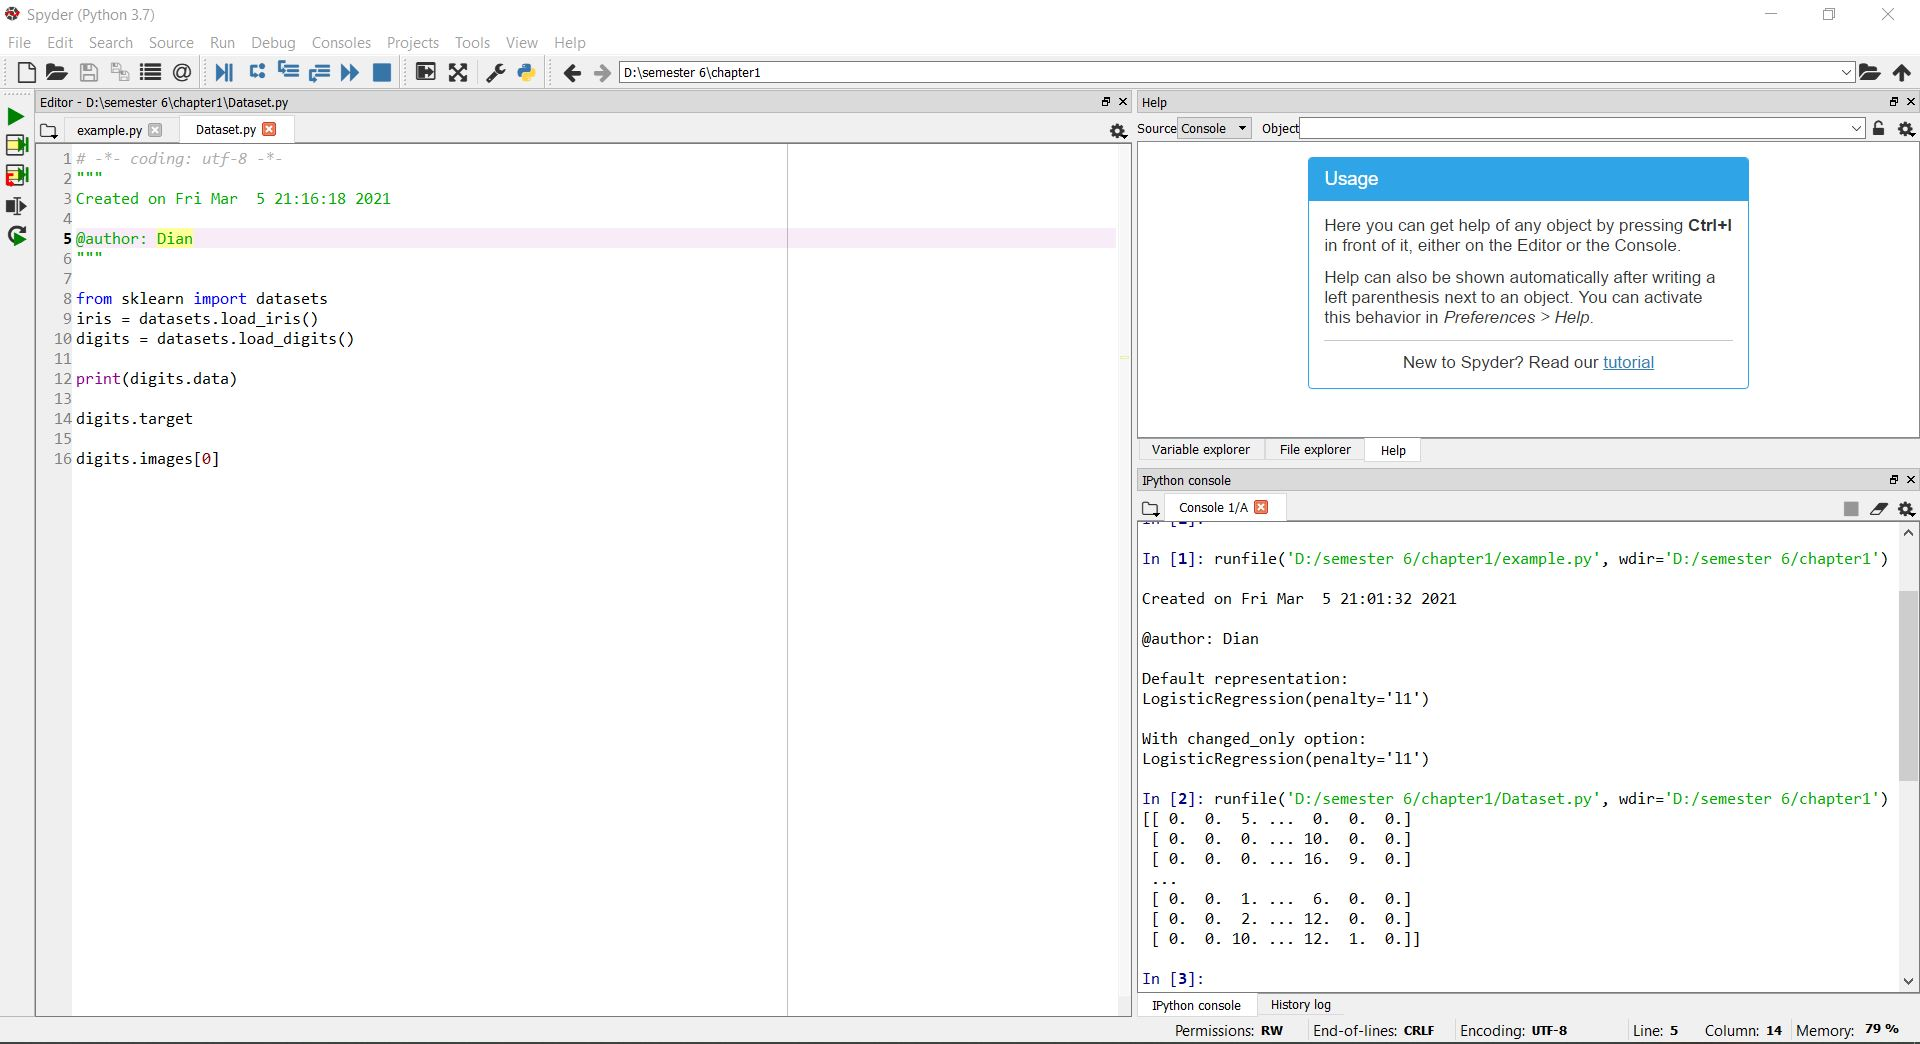
\includegraphics[width=1\textwidth]{figures/1184095/chapter1/6.JPG}
		\caption{example dataset}
		\label{print}
		\end{figure}
		
		\textbf{Penjelasan koding} :
		
		
		\begin{verbatim} from sklearn import datasets \end{verbatim} script diatas maksudnya import class dataset dari scikit learn library
		
		\begin{verbatim} iris = datasets.load_iris() \end{verbatim} script diatas menunjukkan dataset iris dimuat dan dimasukkan  ke variable bernama iris
		
		\begin{verbatim} digits = datasets.load_digits() \end{verbatim} script diatas menunjukkan  dataset digits dimuat dan dimasukkan ke variable digits
		
		\begin{verbatim} print(digits.data) \end{verbatim} memberi akses ke fitur yg dipakai untuk mengklasifikasi sampel digits 
		
		\begin{verbatim} digits.target  \end{verbatim} merupakan info data label
		
		\begin{verbatim} digits.images[0]  \end{verbatim} Merupakan data yang berupa array 2D, shape(n.samples. n.features), walaupun data aslinya bisa berbeda bentuk.
		
		\item{latihan berikutnya mencoba learning and predicting}
        \begin{figure}[H]
		\centering
		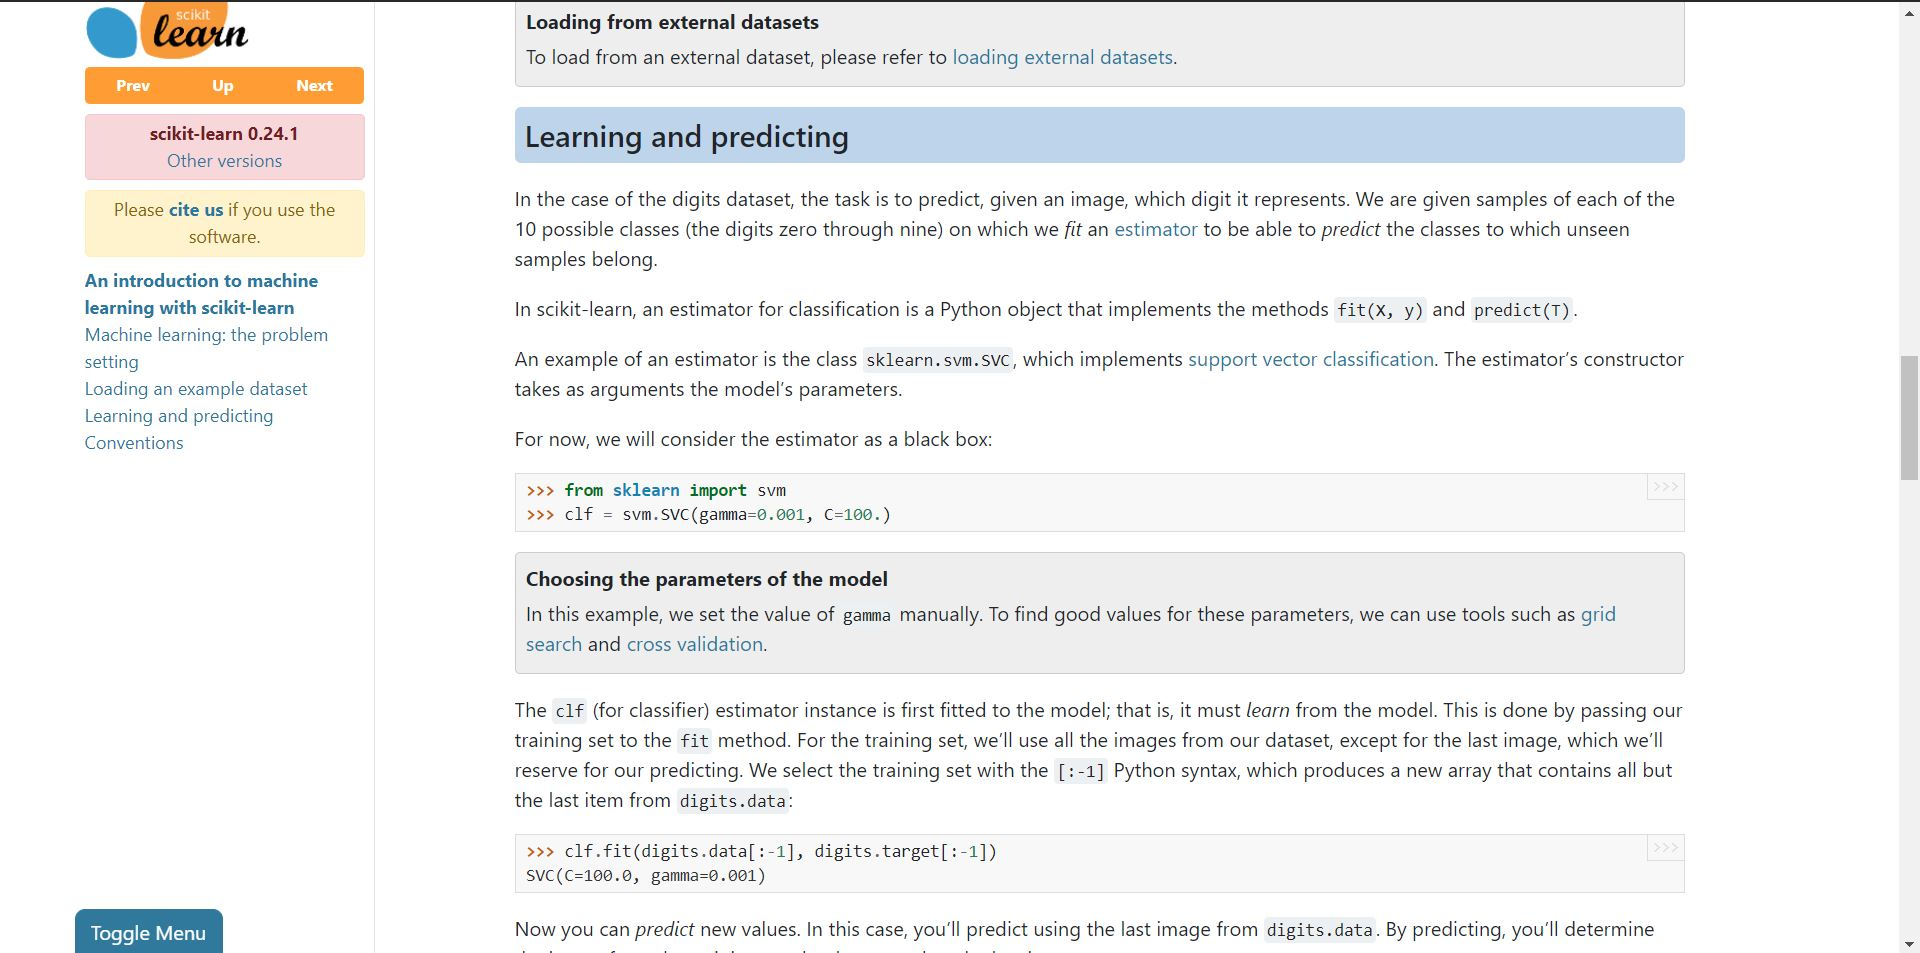
\includegraphics[width=1\textwidth]{figures/1184095/chapter1/7awal.JPG}
		\caption{example learning and predicting}
		\label{print}
		\end{figure}
		
		\item{Jalankan dan lihat hasilnya}
        \begin{figure}[H]
		\centering
		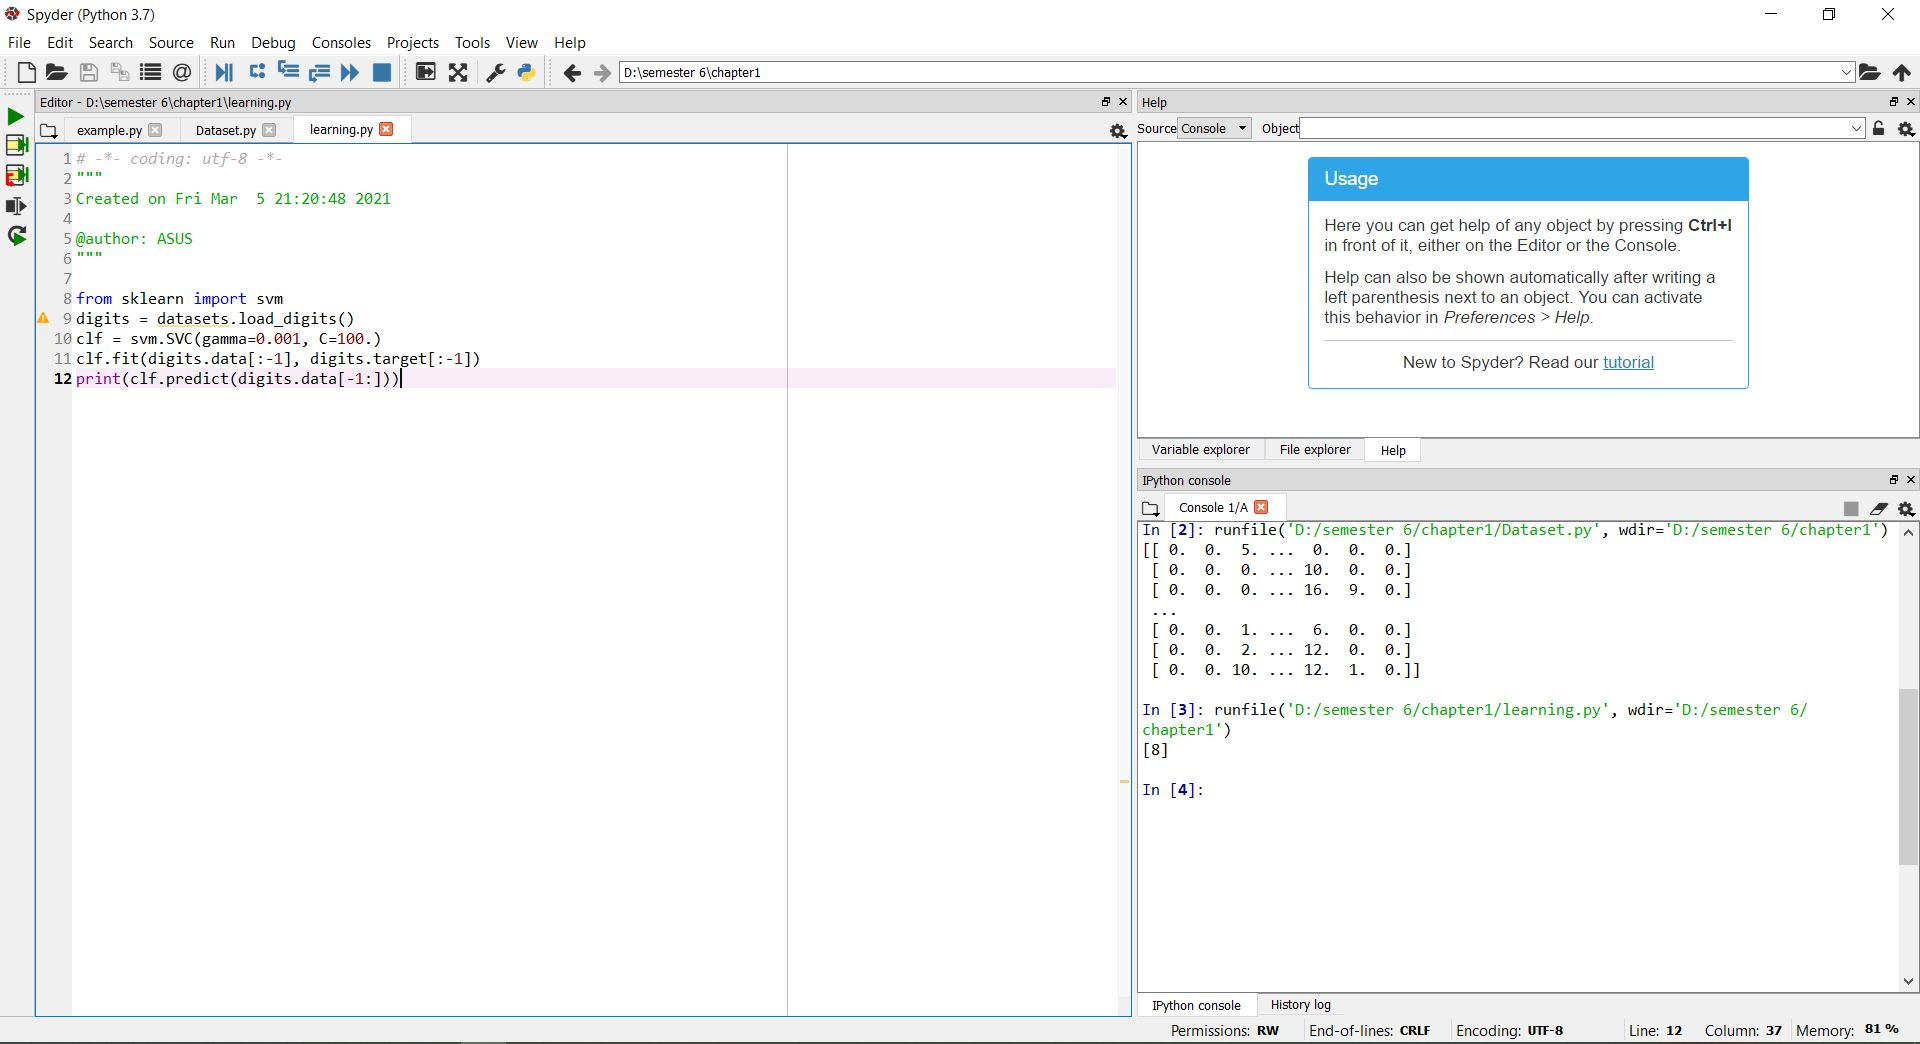
\includegraphics[width=1\textwidth]{figures/1184095/chapter1/7.JPG}
		\caption{example learning and predicting}
		\label{print}
		\end{figure}
		
		\textbf{Penjelasan koding} :
		
		
		\begin{verbatim} from sklearn import svm \end{verbatim} script diatas maksudnya import class class svm dari package sklearn.
		
		\begin{verbatim} digits = datasets.load_digits() \end{verbatim} script diatas menunjukkan  dataset digits dimuat dan dimasukkan ke variable digits
			
		\begin{verbatim} clf = svm.SVC(gamma=0.001, C=100.)  \end{verbatim} clf sebagai estimator/parameter. svm. kemudian SVC sebagai class nya dan gamma sebagai parameter untuk penetapan nilai yang dilakukan secara manual

		
		\begin{verbatim} clf.fit(digits.data[:-1], digits.target[:-1])  \end{verbatim} clf sebagai estimator/parameter. fit sebagai metode nya kemudian digits.data sebagai item dan [:1] sebagai syntax python yang menampilkan output.
		
		\begin{verbatim} print(clf.predict(digits.data[-1:]))  \end{verbatim} clf sebagai estimator/parameter. predict sebagai metode lain. digits.data sebagai item dan menampilkan output.
		
		\item{latihan selanjutnya mencoba Model persistence}
        \begin{figure}[H]
		\centering
		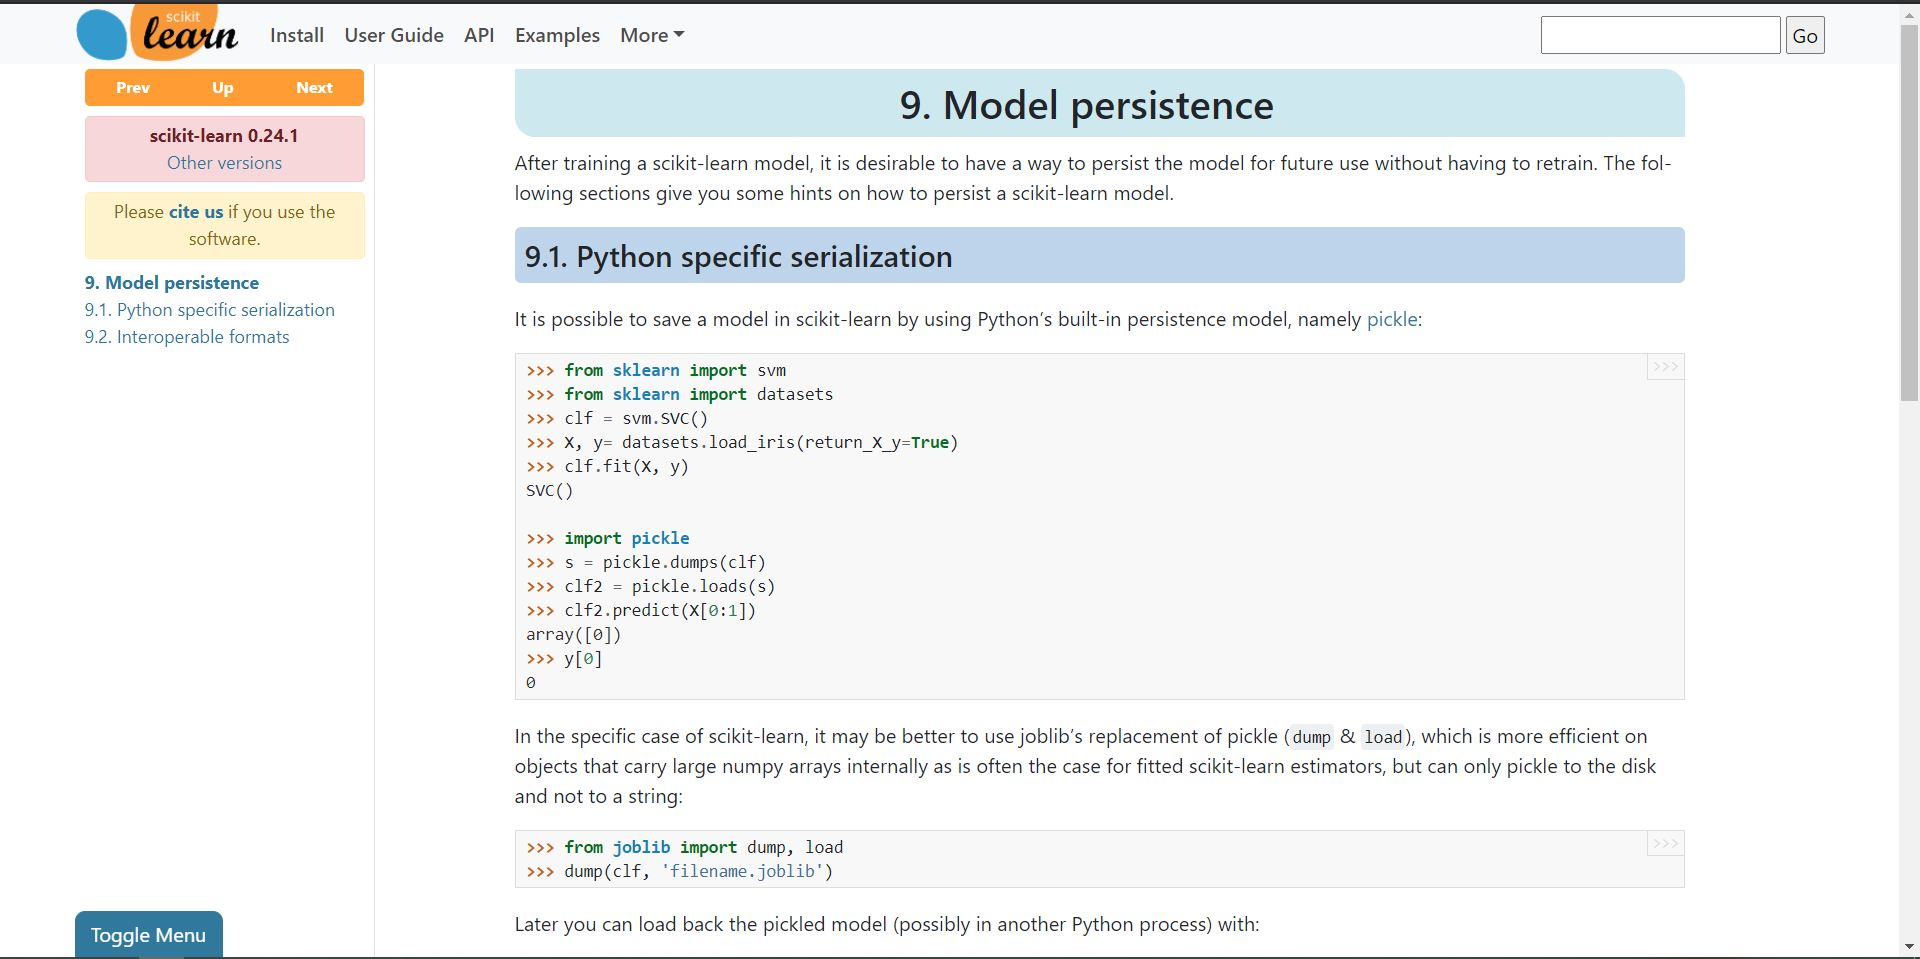
\includegraphics[width=1\textwidth]{figures/1184095/chapter1/9 awal.JPG}
		\caption{example model persistence}
		\label{print}
		\end{figure}
		
		\item{Jalankan dan lihat hasilnya}
        \begin{figure}[H]
		\centering
		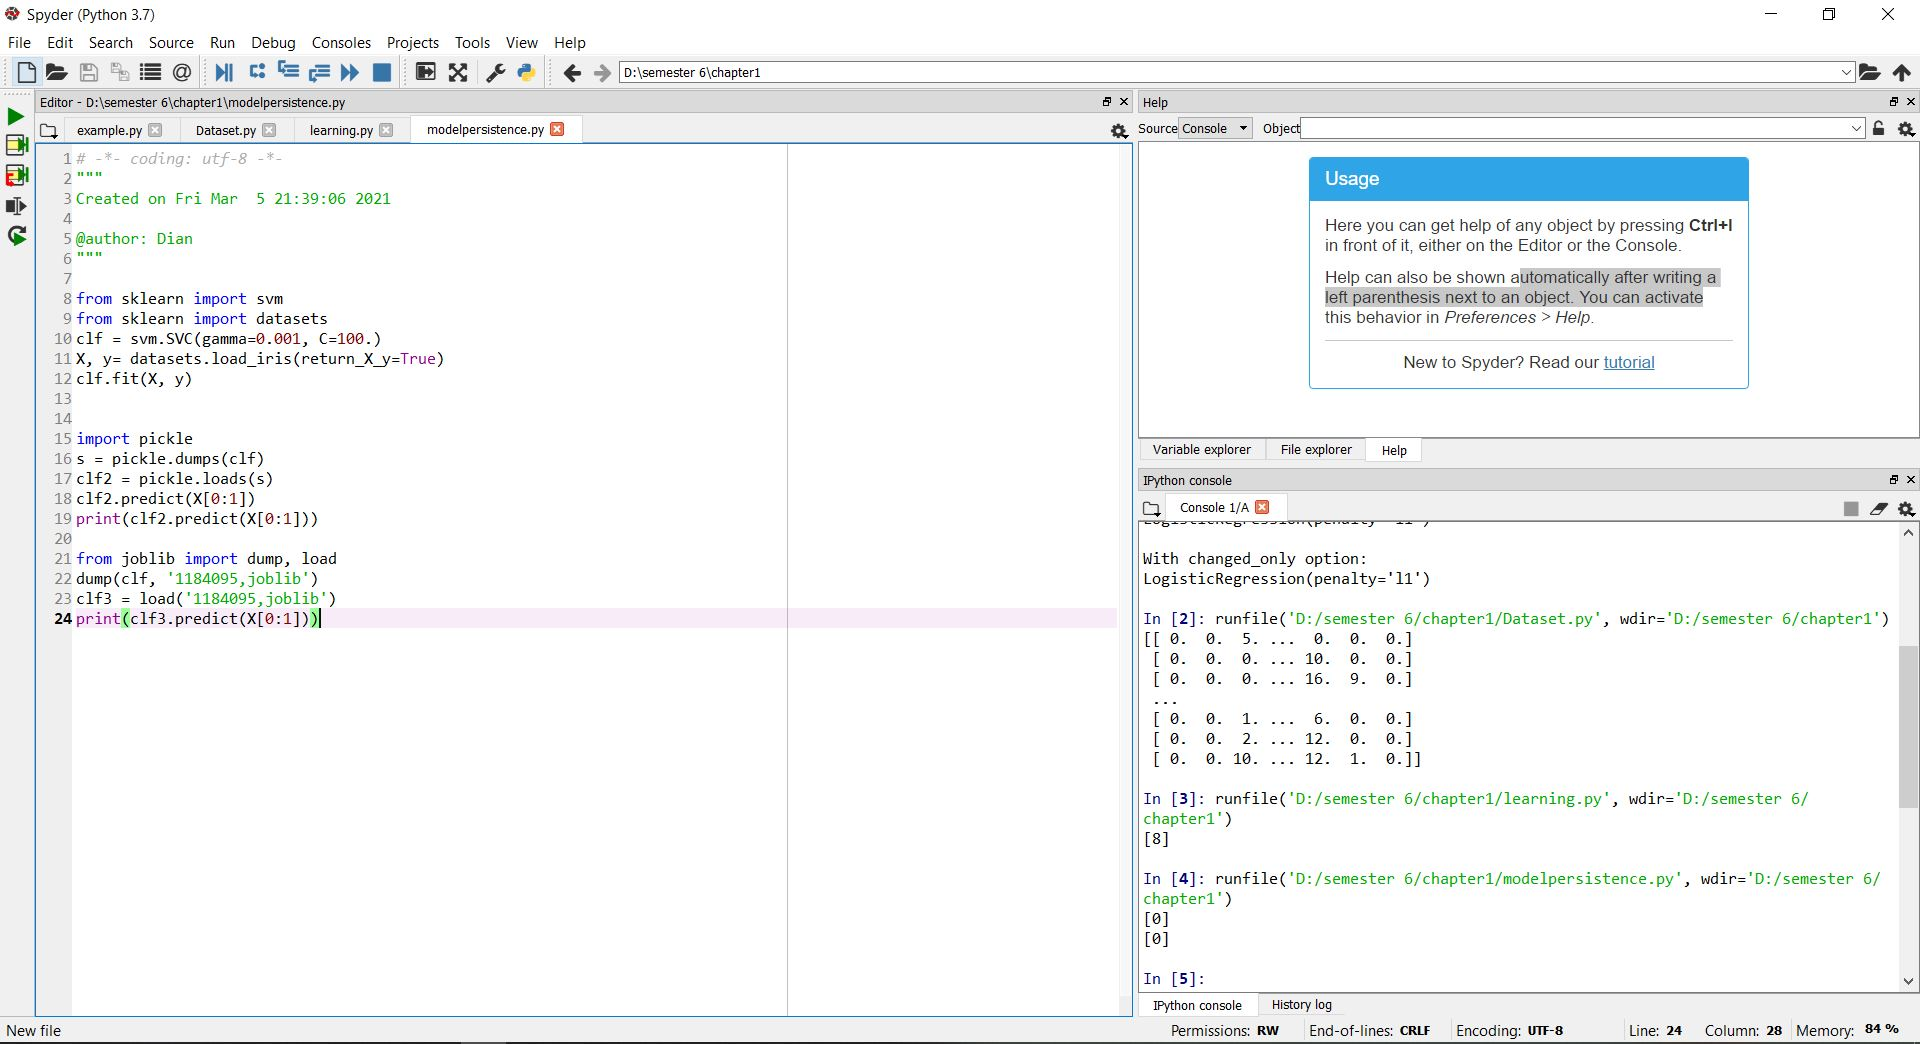
\includegraphics[width=1\textwidth]{figures/1184095/chapter1/9.JPG}
		\caption{example model persistence}
		\label{print}
		\end{figure}
		
		\textbf{Penjelasan koding} 
		
		\begin{verbatim}from sklearn import svm\end{verbatim}import svm dari scikit learn library
		
		\begin{verbatim}from sklearn import datasets\end{verbatim}import dataset dari scikit learn library
        
        \begin{verbatim}clf = svm.SVC(gamma=0.001, C=100.)\end{verbatim} memanggil class SVC dan manset argument sonstructor SVC serta ditampung di variable clf
        
        \begin{verbatim}X, y= datasets.load_iris(return_X_y=True) \end{verbatim}meload dataset iris dan datasets dan ditampung di variable x untuk data dan y untuk target

        \begin{verbatim}clf.fit(X, y)\end{verbatim}memanggil methode fit untuk melakukan training data dengan argumen data dan target dari datasets iris

        \begin{verbatim} import pickle\end{verbatim} mengimport pickle
        
        \begin{verbatim} s = pickle.dumps(clf) \end{verbatim} memanggil method dumps dengan argumen clf dan ditampung di variable s
        
        \begin{verbatim} clf2 = pickle.loads(s)\end{verbatim} memanggil metnode loads dengan argumen s dan ditampung di variable clf2
        
        \begin{verbatim} print(clf2.predict(X[0:1]))\end{verbatim}menampilkan hasil dari method predict dengan argumen data variable

        \begin{verbatim}from joblib import dump, load\end{verbatim} mengimport dump dan load dari library joblib dump(clf, '1184095.joblib') ini untuk memanggil methode dumps dengan argumen clf dan nama file joblibnya
        
        \begin{verbatim} clf3 = load('1184095.joblib') \end{verbatim} memanggil methode loads dengan argumen nama file joblibnya dan ditampung di variable clf3
        
        \begin{verbatim}print(clf3.predict(X[0:1]))\end{verbatim}menampilkan hasil dari methode predict dengan argumen data variable x pertama
        
        \item Latihan berikutnya mencoba Conventions
        \begin{figure}[H]
		\centering
		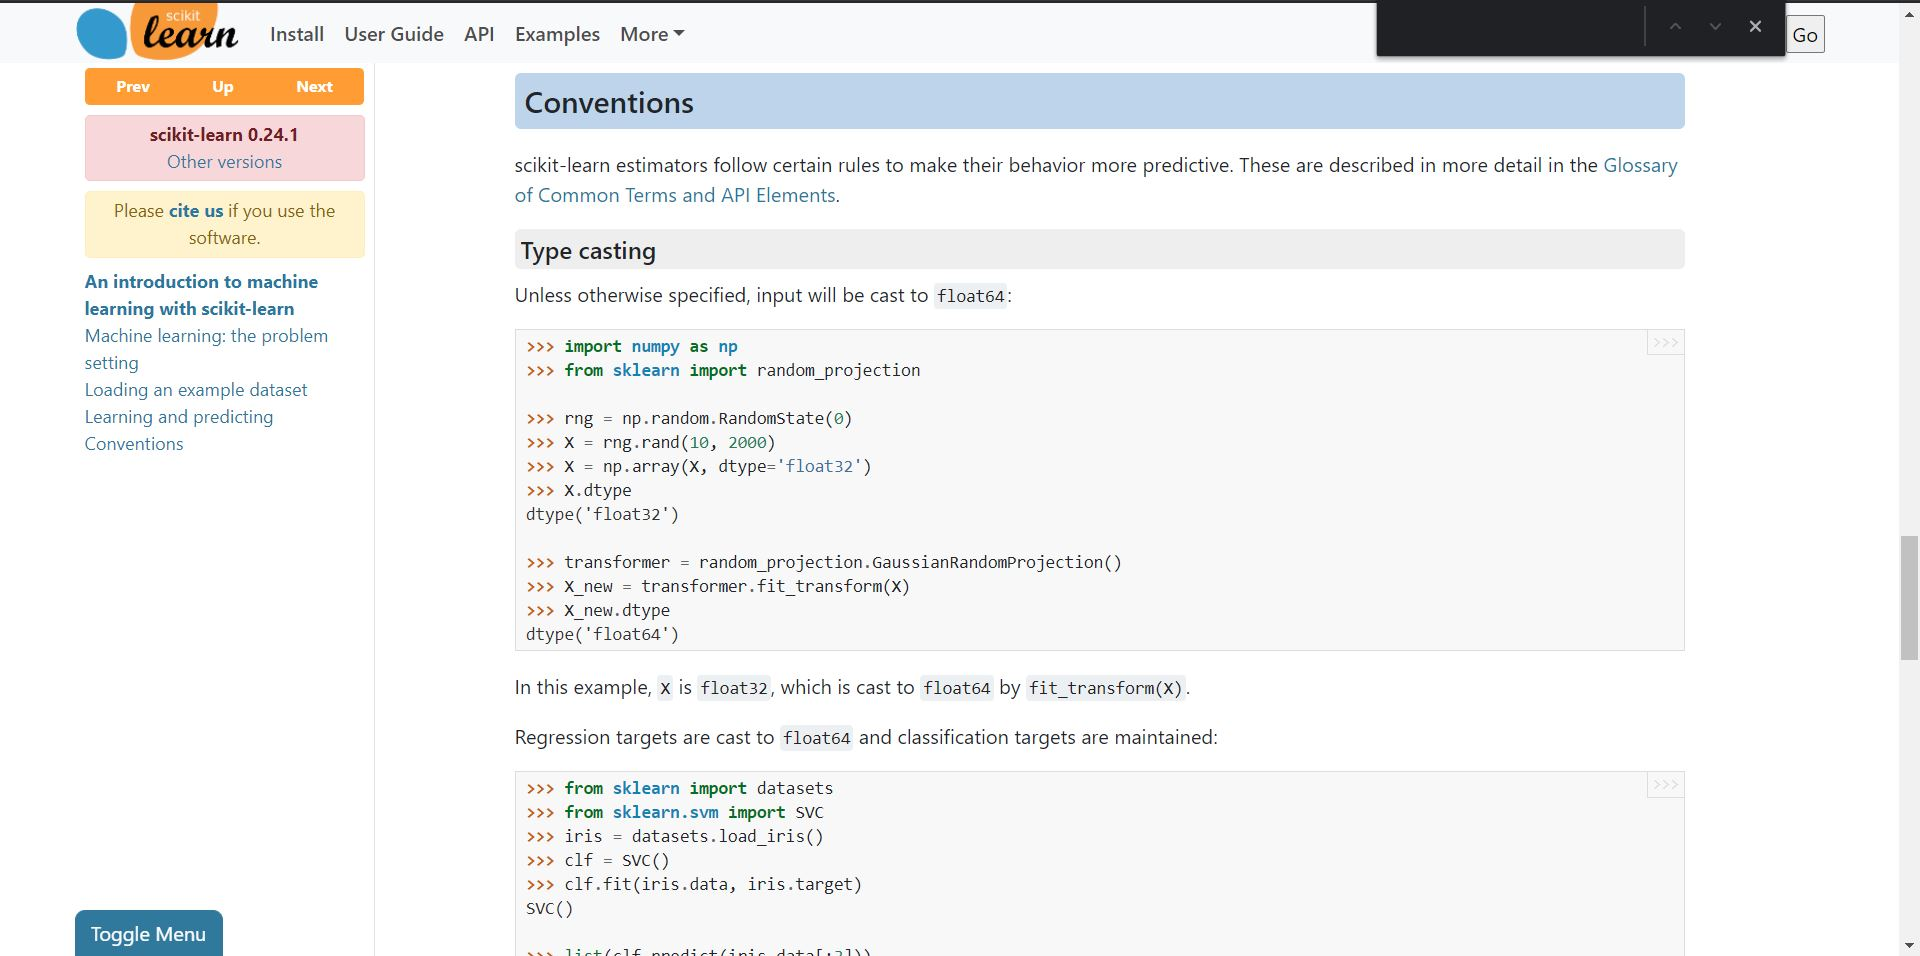
\includegraphics[width=1\textwidth]{figures/1184095/chapter1/10 awal.JPG} 
		\caption{Conventions}
		\label{print}
		\end{figure}
	
        \item Jalankan dan lihat hasilnya
        \begin{figure}[H]
		\centering
		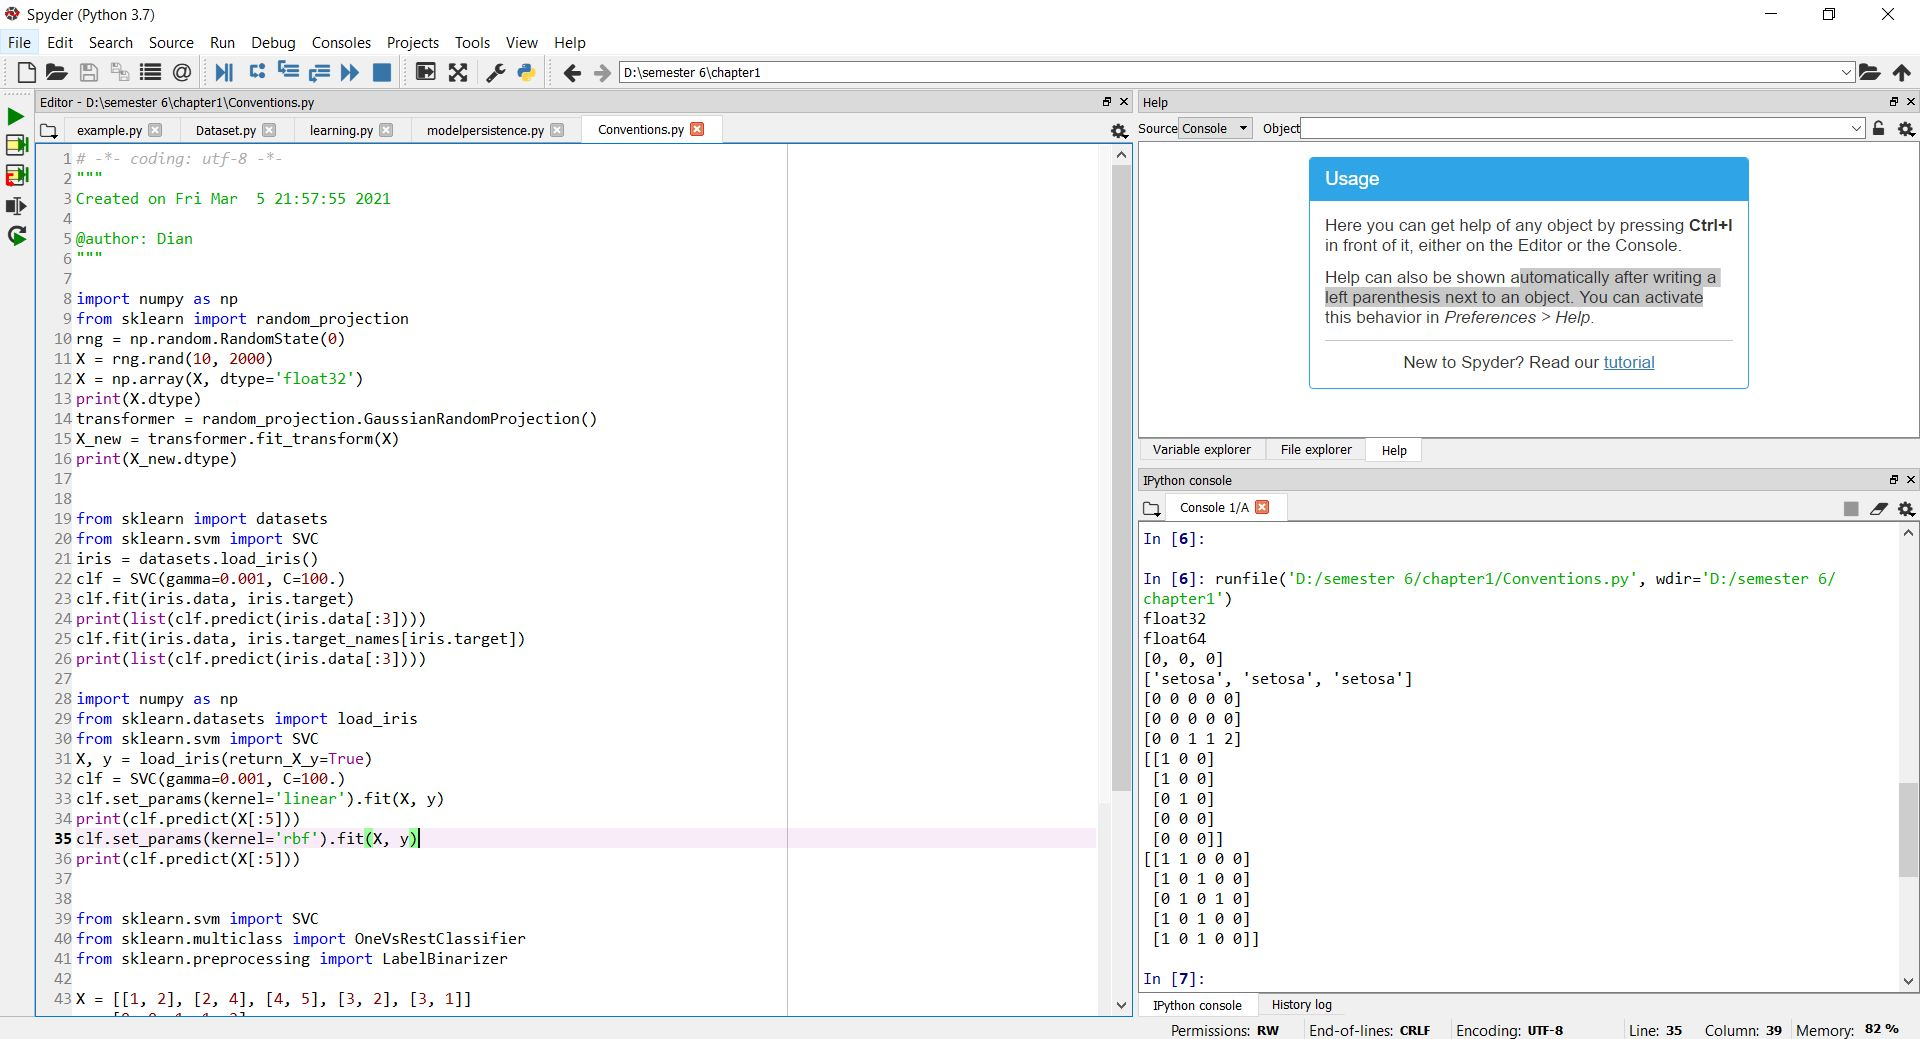
\includegraphics[width=1\textwidth]{figures/1184095/chapter1/11.JPG} 
		\caption{example Conventions}
		\label{print}
		\end{figure}
		
        \begin{figure}[H]
		\centering
		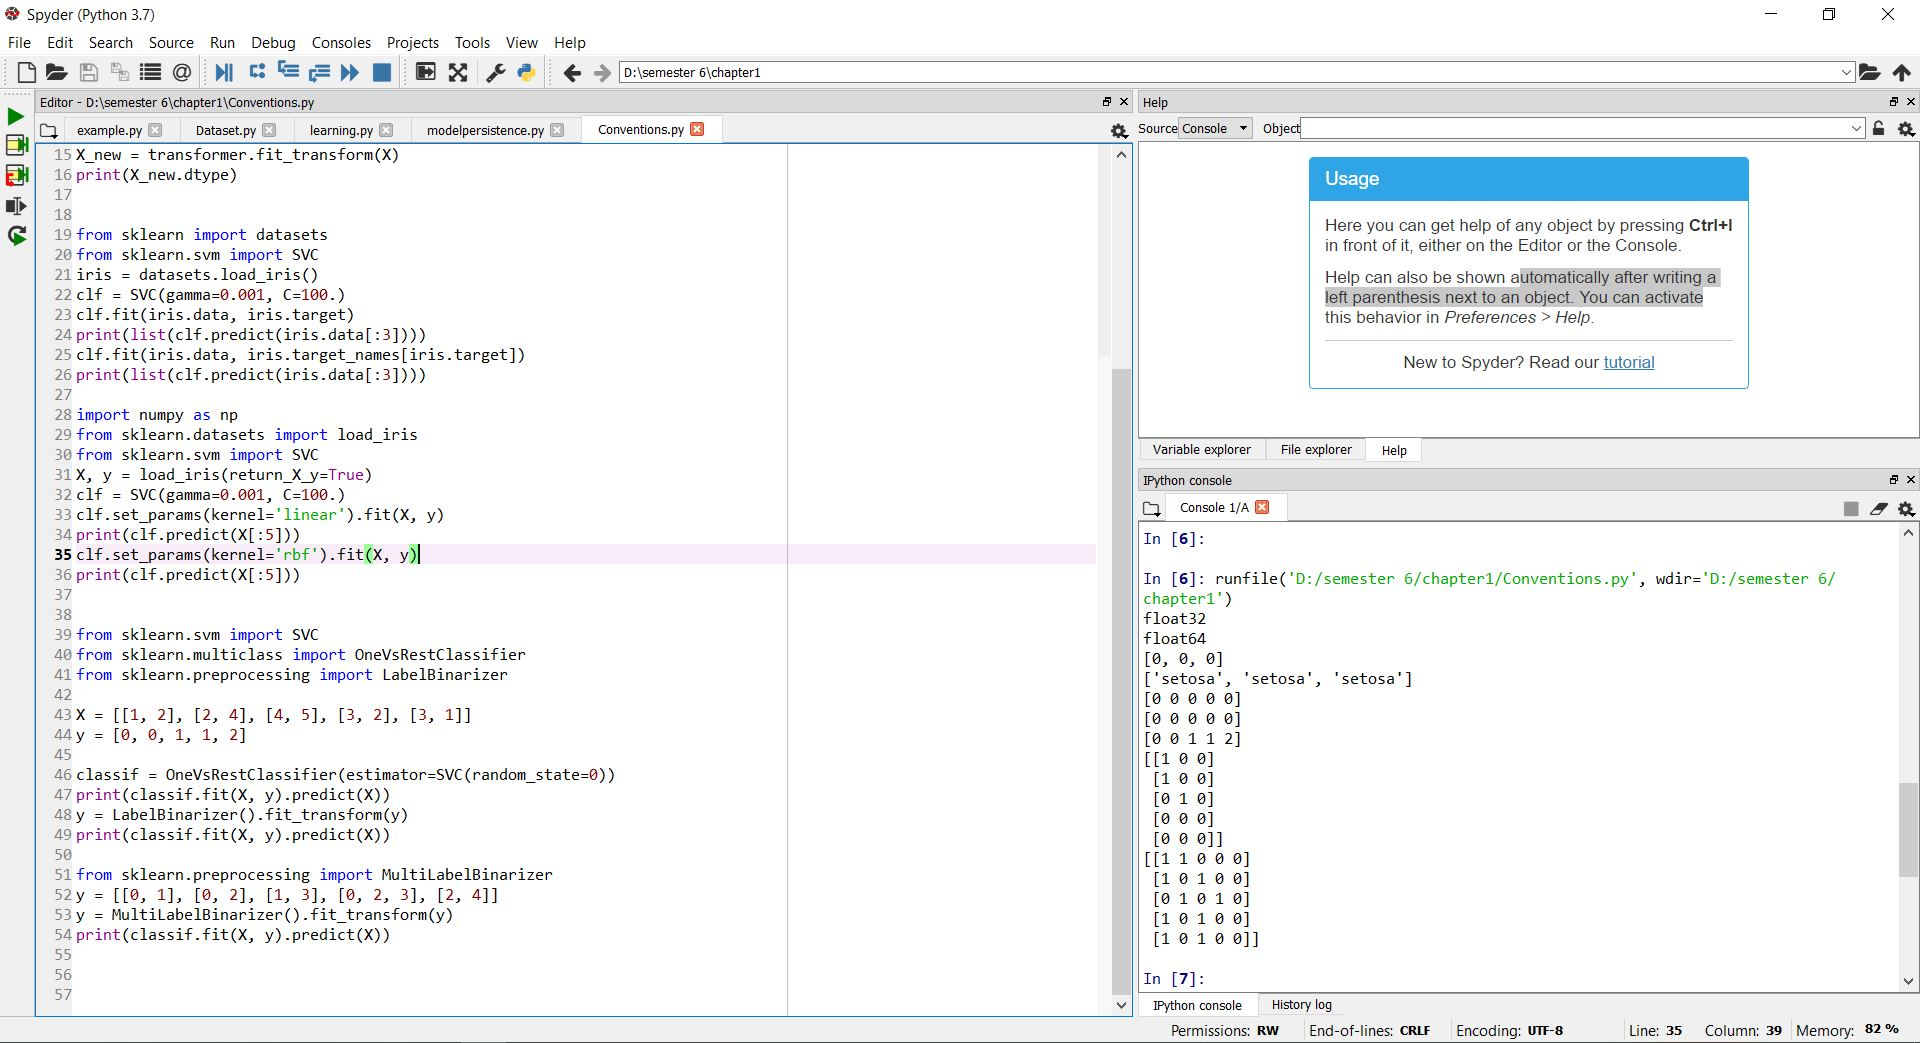
\includegraphics[width=1\textwidth]{figures/1184095/chapter1/11 part 2.JPG}
		\caption{example Conventions part II}
		\label{print}
		\end{figure}
\end{enumerate}

\subsection{Error dan Solusinya}
\begin{enumerate}
		\item Screenshoot Error
		\begin{figure}[H]
		\centering
		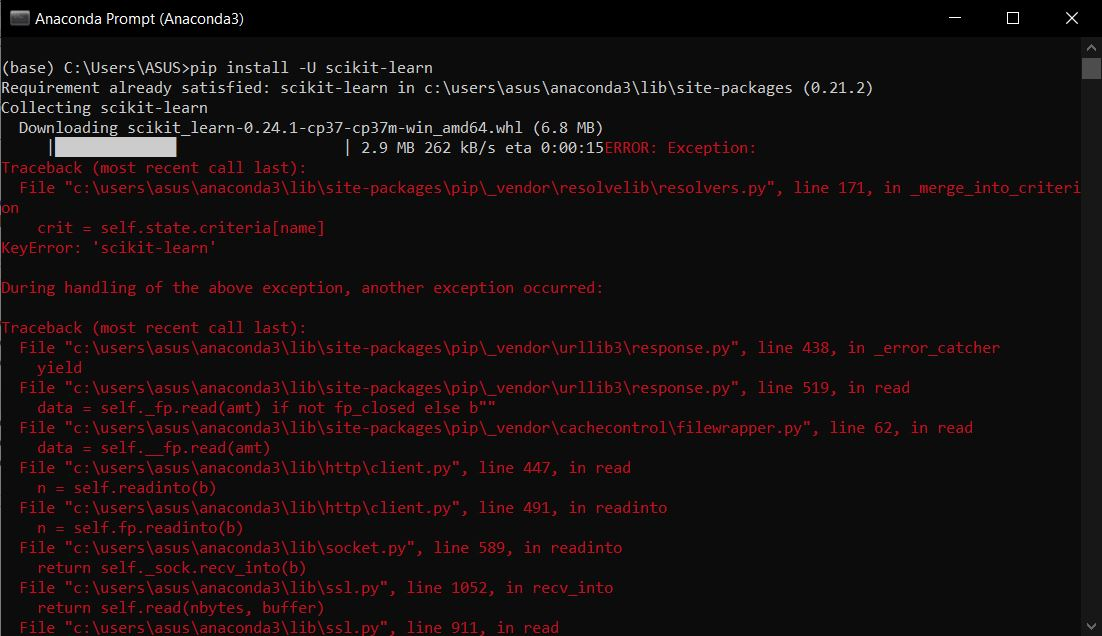
\includegraphics[width=1\textwidth]{figures/1184095/chapter1/eror install.JPG}
		\caption{Error 1}
		\label{print}
		\end{figure}
		
		

		\begin{figure}[H]
		\centering
		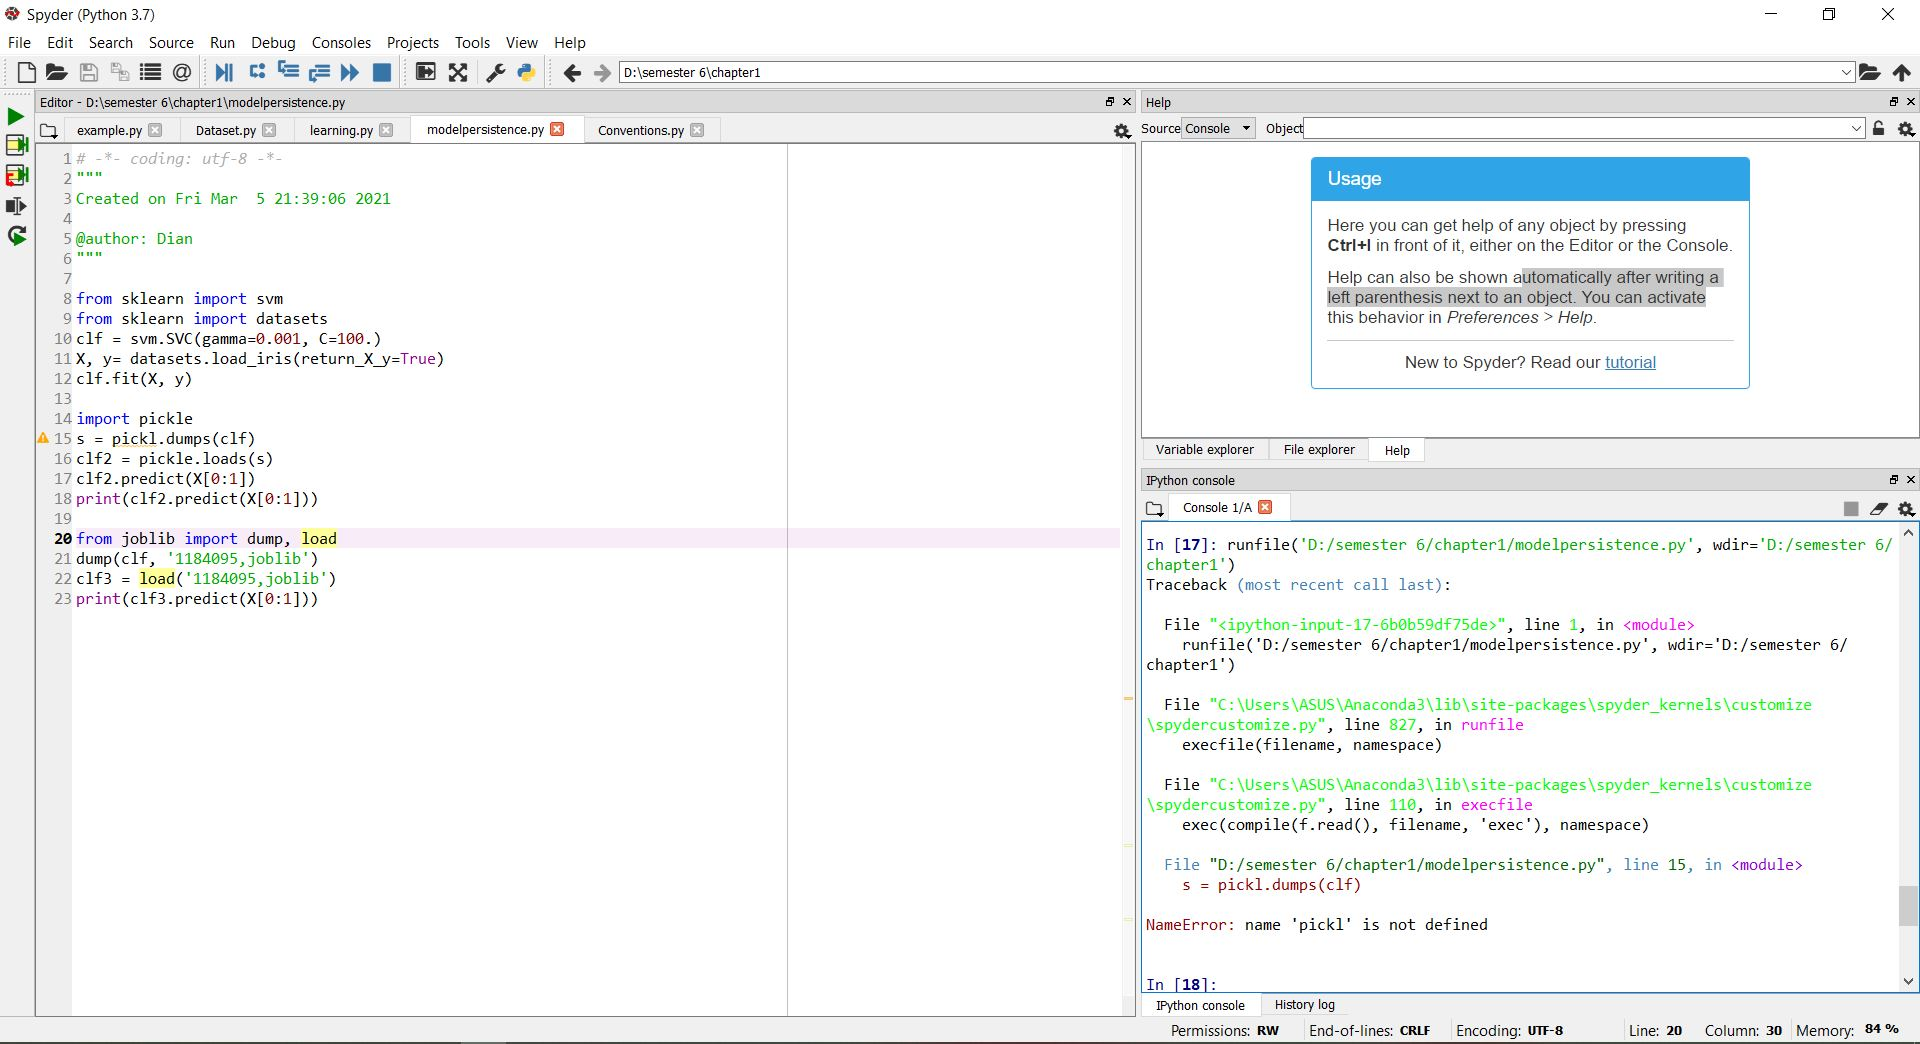
\includegraphics[width=1\textwidth]{figures/1184095/chapter1/eror 2.JPG}
		\caption{Error}
		\label{print}
		\end{figure}
		
		\item Kode dan Jenis error
		
			\subitem \textit{is not defined}, pickl tidak terdefinisi sehingga tidak bisa dipanggil.
			
			

		\item Solusi penanganan error
		
		    \subitem Solusi eror installasi adalah pastikan koneksi yang terhubung ke Laptop/ koneksi harus stabil
		    
			\subitem Solusinya pastikan variabel yang dipanggil ada atau tidak typo. 
			
			
	
		
	\end{enumerate}
\end{document}
